\documentclass[10pt]{article}
\usepackage{graphicx} % Required for inserting images
\usepackage{url}
\usepackage{hyperref}
\title{IEG_Problems_Lecture1}
\author{martavictoriaperez }
\date{March 2025}

\usepackage[margin=1in]{geometry} 
\usepackage{amsmath,amsthm,amssymb, graphicx, multicol, array}
 
\newcommand{\N}{\mathbb{N}}
\newcommand{\Z}{\mathbb{Z}}
 
\newenvironment{problem}[2][Problem]{\begin{trivlist}
\item[\hskip \labelsep {\bfseries #1}\hskip \labelsep {\bfseries #2.}]}{\end{trivlist}}

\begin{document}
 
\title{\textbf{Lecture 6: Gas networks}}
\author{
%Your name\\
DTU Course 46770: Integrated Energy Grids }
\maketitle

\begin{problem}{6.1}

Consider the simplified network plotted in Fig. \ref{fig_network}, which represents Denmark and its neighbouring countries. Assume that the nodes are connected using transmission methane gas pipelines.

\begin{figure}
    \centering
    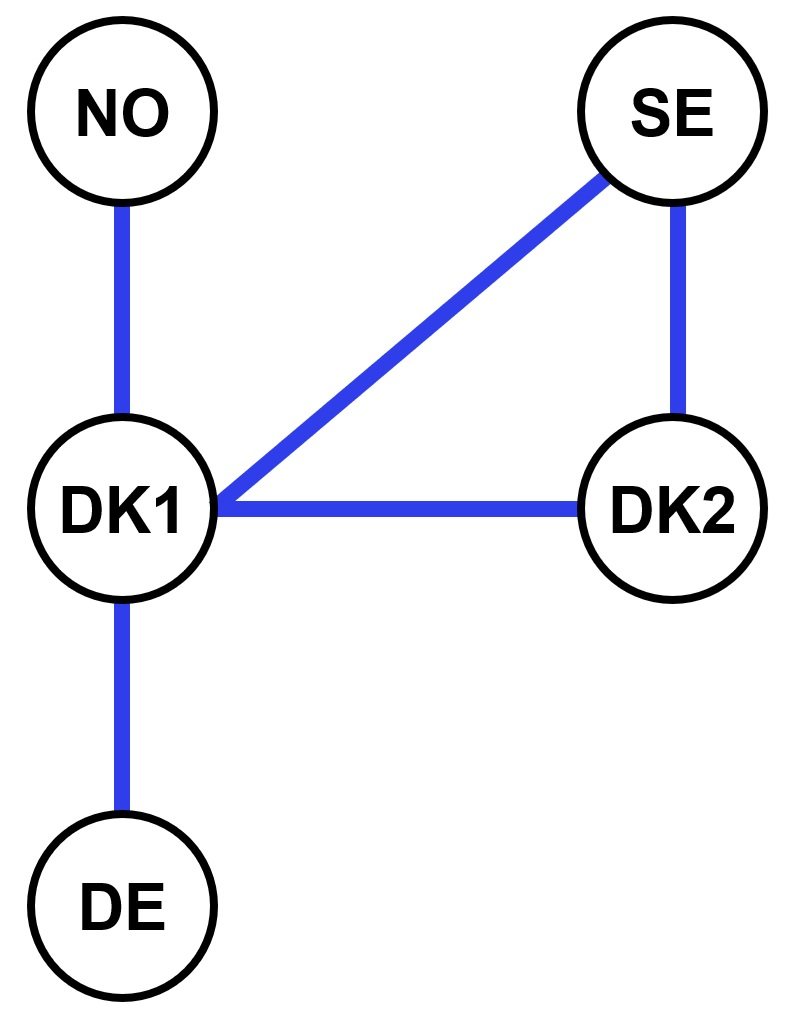
\includegraphics[width=0.2\linewidth]{figures/nodes.jpg}
    \caption{Simplified network.}
    \label{fig_network}
\end{figure}
\begin{itemize}

\item[a)] Calculate the capacity of every pipeline (in MW) assuming that they operate at a pressure $P$=50 bar, the average gas flow velocity is $u$ = 15 m/s, the diameter of the pipes is $D$ = 600mm and the energy content of methane is 50 GJ/tonne. To calculate the speed of sound in gas $c$, assume the universal gas constant $R$=8.314 J/molK, the molar mass of methane $M$=16 g/mol, compression factor $Z$=1.31, and temperature T=25$^{\circ}$C.

\item[b)] Assuming steady-state conditions, use link elements in PyPSA to build a network like the one shown in Fig. 1.  Assume that, in the first time step,  in every node, there is a demand for 1 GWh of methane.  Assume also that, in the Norway node there is a gas generator with a marginal cost of 20 EUR/MWh$_{th}$. Calculate the optimal gas flows through the network and plot them.

\item[c)] Assume now the following lengths for the links: DK1-DK2=200 km, DK1-DE=600 km, DK1-NO= 500 km, DK1-SE=600 km, DK2-SE=100 km. If we consider that the losses due to the compressors' energy consumption to maintain the pressure can be estimated at 2\% of the energy flow per 1000 km. Adapt the link elements in PyPSA to include an efficiency that takes compressors' energy demand into account. Calculate the optimal gas flows through the network and plot them.

\item[d)] Assuming the following demands in GWh for three consecutive time steps DE=[0,0,3], DK1=[1,2,1], DK2=[1,1,1], NO=[1,1,1], SE=[0,1,0]. Calculate the optimal flows in every time step and the total system costs. 

\item[e)] Modify the demand for the German node to be DE=[0,0,6] GWh and keep the other node as in the previous section. Calculate the optimal flows in every time step and the total system costs.

\item[f)] Assume that the pipeline pressure can be increased from 50 to 55 bar, calculate the linepack, i.e., the energy that can be stored in every pipeline by increasing the pressure. Represent this in your PyPSA model by adding a store with that capacity at the beginning of every line, calculate the optimal gas flows in every time step and the total system costs.

\end{itemize}


\end{problem}

\

\begin{problem}{6.2}
Let us assume that the countries in Problem 6.1 are considering repurposing their methane gas network into a hydrogen network. In order to run the existing pipelines with hydrogen, the pressure needs to be reduced to $P$=40 bar, and the average flow velocity can be increased to $u$ = 30 m/s. Calculate the capacity of every pipeline (in MW), and relative to their initial design when they transport methane gas. 

\

The energy content of $H_2$ is 120 GJ/tonne. To calculate the speed of sound in hydrogen $c$, assume the universal gas constant $R$=8.314 J/molK, the molar mass of hydrogen $M$=2 g/mol, compression factor $Z$=1.03, and temperature T=25$^{\circ}$C.


\end{problem}

\

\begin{problem}{6.3}

Assume the gas transport system that is shown in Figure \ref{fig_gas_network}. Gas can be injected in Node 1 at a marginal price of 10 EUR/kg or at Node 5 at 15 EUR/kg. There is a demand of 2$\cdot 10^8$ kg/s in Node 3. Finally, Node 2-3 represents a pumping station where gas pressure can be increased by $k_{23}$=1.2 at a cost that is proportional to the mass flow $m_{23}$  by a constant $o_{23}$ =5 EUR/kg.

\

To calculate the speed of sound in gas $c$, assume the universal gas constant $R$=8.314 J/molK, the molar mass of methane $M$=16 g/mol, compression factor $Z$=1.31, and temperature T=25$^{\circ}$C. Assume the diameter of the pipelines is $D$ = 1000mm, the length $L_{12}$=$L_{34}$=$L_{45}$=100km, and calculate the Darcy friction  coefficient $f_{D}$ assuming fully-turbulent flow and roughness $\epsilon$=0.001m. 

\begin{itemize}

\item[a)] Write the equations of the optimization problem that minimizes the total system cost and use the Weymouth equation to represent pressure drop in the pipelines as a function of the mass flow $m_{ij}$.


\item[b)] Use gurobipy to formulate and solve the problem


\end{itemize}

\begin{figure}[h]
    \centering
    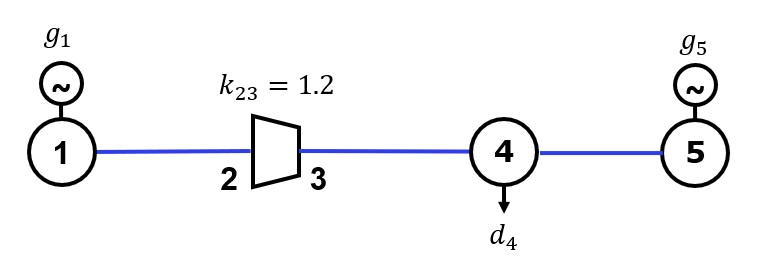
\includegraphics[width=0.6\linewidth]{figures/gas_network.jpg}
    \caption{Gas network.}
    \label{fig_gas_network}
\end{figure}

\textit{Hint: It is recommended to follow the} \href{https://martavp.github.io/integrated-energy-grids/intro-gurobipy.html#}{Gurobipy tutorial} \textit{before trying this problem.}
\end{problem}

%\begin{proof}[Solution]
%Write a solution here
%\end{proof}

\end{document}


 

